\documentclass[a4paper, oneside]{report}

\usepackage[vlined, ruled, linesnumbered]{algorithm2e}
\usepackage{amsmath}
\usepackage{fancyref} % Better reference.

\usepackage{pdflscape} % Gør landscape-environmentet tilgængeligt
\usepackage{fixme} % Indsæt "fixme" noter i drafts.
%\usepackage{hyperref} % Indsæter links (interne og eksterne) i PDF

\usepackage[format=hang]{caption,subfig}
\usepackage{graphicx}
%\usepackage{stmaryrd}
\usepackage{amssymb}
%\usepackage{listings}
%\usepackage{ulem} % \sout - strike-through
%\usepackage{tikz}
\renewcommand{\ttdefault}{txtt} % Bedre typewriter font
\newcommand{\keyword}{\ttfamily}
\newcommand{\STL}{STL (C++ Standard Template Library)}

\setcounter{secnumdepth}{-1} % Sæt overskriftsnummereringsdybde. Disable = -1.
\newcommand{\projecttitle}{Implementing and parallelising Bursttries}

\title{\projecttitle}
\author{Jacob Wejendorp}
%\renewcommand{\bibsection}{\section*{References}}
\begin{document}
\maketitle
\noindent
{\bf Abstract}
\\\\
With the scaling of CPUs focusing more on increases in the number of cores,
highly parallelisable data structures are of increasing importance.

This project seeks to explore the implementation tradeoffs in parallelising the
burst trie data structure, which has been shown to be on par with hash maps in
both speed and space consumption. The burst trie provides fast access to
strings and integers, however different bucket types have different advantages
and disadvantages.

By comparing different tradeoffs needed to implement partial functionalities,
specialized data structures are developed. Depending on the level of
parallelism, distribution of insertions/searches/removals, and the
distribution of the inserted data, different variations excel. This means
evaluating the modifications needed to make the trie work as a threadsafe set-,
multiset- or map container.

The performance of the trie in sequential testing is found to degrade with
increased bucket sizes, while the opposite tendency is found for parallel
scaling for larger datasets. As such no silver bullet is found for bucket
sizes.

Using a relatively simple locking mechanism, speedups of up to a factor $6$ are
observed for searches and $3.5$ for insertions, when utilizing 8 CPUs.

A lock-free implementation technique is proposed to avoid bottlenecking at the
root of the trie, but not successfully implemented.
\\\\
{\bf Resume}
\\\\
Da skalering af processorer i stigende grad fokuserer på forøgelse af antallet af
kerner, er højt paralleliserbare data strukturer af stigende vigtighed.

Dette projekt søger at undersøge hvilke kompromiser der indgår i implementation
af burst trie datastrukturen, der er vist at være på højde med hash maps
både med ydelse og hukommelses forbrug. Burst trien giver hurtig tilgang til
strenge og heltal, men forskellige bucket typer har forskellige fordele og ulemper.

Ved at sammenligne de forskellige kompromiser nødvendige for at implementere dele
af funktionaliteten udvikles specialiserede datastrukturer. Afhængig af niveauet
af parallelisme, fordeling af indsættelser/søgninger/sletninger, og fordeling
af det indsatte data, vil forskellige variationer være bedst. Dette betyder at
vi må evaluere modifikationerne der er nødvendige for at gøre strukturen til
en trådsikker sæt-, multisæt- og map struktur.

Ydelsen for trien ved sekventiel test ses at gå ned med forøgede bucket størrelse
mens den omvendte tendens ses for parallel skalering for større datasæt. Derfor
findes der ingen gylden bucket stoerrelse.

Med brug af relativt simple locking metoder, observeres speedups på op til en
faktor 6 for søgninger og 3.5 for indsættelser med brug af 8 processorer.

En lock-free implementation foreslås for at undgå flaskehalse ved
roden af trien, men har ikke kunnet implementeres.


\clearpage

\tableofcontents*
\clearpage

\chapter{Introduction}

\section{Problem definition}
How can the burst trie be parallelised, in a way that allows building and searching
the structure faster than an equivalent serial singlethreaded approach?
What kind of overhead does it create, and does this influence relative
performance between the individual variants of the structure?


\section{Background}
%Define: What is a trie?
A trie is a datastructure for storing keys based on their prefixes.
It is also known as a prefix-tree. The idea is equivalent to that of
"most significant digit" (MSD-)radix sort.

Each level in the tree reads a prefix of the key and branches accordingly.
A trie working on strings with the ASCII alphabet will thus have a branching
factor of 128. Each read character corresponds to a branch and goes down another
level until finding the leaf matching the requested key or terminating
unsuccesfully. A trie is as deep as the longest key that it contains, since
each level removes a character from the key. It is this bound that newer trie
variants attempt to improve, without compromising lookup efficiency.

%Define: What is the idea of a burst trie?
Following the radix sort analogy, the regular trie uses radix-sort until
reaching the trivial case, with no boundary for using other sorting methods.
The burst trie, on the other hand, uses a limit for employing other methods
based on the element count. In other words a burst trie differs from a regular
trie by the fact that it compresses the elements into "bucket" structures when
there are few of them in a particular subtree. Each bucket is then assigned a
capacity. When inserting elements into a burst trie, the structure finds the
corresponding bucket and puts the element in it. If the bucket exceeds its
capacity it "bursts", creating a new parenting node and redistributing the
elements into buckets under it, based on the next part of the prefix. As such,
each bucket is uniquely determined by its prefix (or path), and the elements in
each bucket have the same prefix, making it possible to discard this
information to save space. This is what makes it possible for the trie to be
more space efficient than an equivalent hashmap, or comparison-based tree
structure.

% Why are burst tries nice?
Burst tries have been shown to be faster and more space efficient than
compari\-son-based datastructures such as B-trees and red-black trees when used
on integer data. For strings the burst trie is more efficient than trees, while
unlike hash-tables allowing efficient iteration of sorted keys with minor
modifications. In that context it would be interesting to see how versatile the
structure is, if it is able to compete with other {\keyword (multi-)set}
structures and heaps with relevant modifications.

The original burst trie uses linked lists for the containers, but this has been
shown to be inefficient in a modern cache hierachy. There has been done research
in different ways to improve the structure, by replacing the bucket structure.
Nash and Gregg have done work on optimizing the trie itself, using so-called
level- and path-compression.\cite{Nash:2008}

In an earlier course, the author has done work on the burst trie as an Integer
datastructure in cooperation with Niels Grathwohl. Here, a simplistic
bit-string approach was used to allow different datatypes in the
branching.\cite{Wejendorp:2010}

% Multithreading!!
While maintaining optimizations for caching remains important, modern processor
scaling primarily focuses on multithreading, making it increasingly important
to create efficient multi-threaded datastructures and algorithms.
To the author's knowledge, no work has been done on parallelising the structure
for modern multi-core processors, as this was left open by Askitis and Sinha.
\cite{Askitis:2010}

%Weaknesses...
Although the burst trie has been studied with respect to cache optimization, no
work has been done in parallelising the structure in a way that allows
insertions and deletions faster than the sequential implementation, while
remaining space efficient\cite{Askitis:2010}. This means evaluating the
sacrifices needed to make the structure threadsafe; the number of locks,
indicator variables and the like.

Parallelism in general is a very complex issue, with cache alignment having a
potentially large impact on performance, from so-called false sharing
\cite{Shavit:2011}. This phenomenon occurs when two cpus operate on the same
memory region, but on independent data, and is the unnecessary synchronization
of cachelines between CPUs.

Another area of interest is minimal locking, which will decrease the amount of
syncrhonization between threads. The standard datastructures of C++ are all
threadsafe in terms of concurrent reads, but not writes. As such, a simple
read/write lock can be used to wrap the structure, causing forced sequential
writing, while allowing multiple readers. [Pthread reference] When locks are
used, the scheduler must guarantee that the threads holding the locks are not
preempted. Otherwise the performance of all waiting threads will suffer. A
solution to this is to try and design a lock-free implementation.

What makes lock-free implementation difficult is potential race conditions from
data dependencies. This is attempted to be resolved using a
mixture of so-called atomic operations, in combination with compare-and-set
(CAS) and contention. Using this method, one operation will always succeed
for every time another fails, and progress is guaranteed regardless of
    what the scheduler does.\cite{Shavit:2011} It is therefore of great interest
    to investigate ways to make the trie lock-free.
Doing so will also ensure operations not being limited in terms of parallelisation
to a factor of the trie breadth at a given level (per-node parallel).

\chapter{Implementation}
By first establishing the regular trie methods, a basis is made for evaluating
the modifications required by the other types. All used structures are
implemented from scratch, unless otherwise noted.

In the analysis of the various containers and the general trie, the following
notation will be used:
% Time bounds
\begin{table}[h!]
    \centering
    \begin{tabular}[here]{ l l}
        Notation & Meaning \\ \hline
        n       & The number of elements.\\
        $\alpha$& The alphabet size, or node size.\\
        b       & The bucket size.\\
        h       & The (maximum-)height of the trie. \\
    \end{tabular}
    \caption{Table of the analysis notation}
    \label{tab:notation}
\end{table}

\section{The trie}
The basic trie creates one node for each unique suffix character of the input string,
and as such will always have the height of the longest string inserted.
The {\keyword insert} method builts the trie using the following algorithm:

\begin{algorithm}[H]
    \caption{Generic trie \FuncSty{Insert(key k)}}
    \label{alg:gt_insert}

    $Node \leftarrow$  root node\;
    \ForEach{char $c$ in $k$}{
        \eIf{$Node$ has child $c$}{
            $Node \leftarrow Node[c]$\;
        }{ %else
            $Node[c] \leftarrow$ \emph{new $Node$}\;
            $Node \leftarrow Node[c]$\;
        }
    }
    \emph{Set end of string flag on $Node$}\;
\end{algorithm}

Using this as the basis for the insertion and deletion methods, the trie is
built and searched by reading one character at a time. So just like an
insertion might create a deep path down the trie, a deletion will have to
remove dead ends upon removing an entry. A depth-first approach is taken
with deletions. The recursive call returns with a value, determining if
changes might be needed at the higher level.

If the trie is used to store (key,value) pairs, the end of string flag is
simply a pointer to the value. The trie operations depend solely on the height,
and insertions, searches and removals are all $O(h)$.

\subsection{Burst trie}
The burst trie uses the same basic methods as outlined above. The child check
"c" is extended to cover two kinds of children instead of just nodes. The
descent condition of the regular trie is to move down until end of string, while
the burst trie will also altered to stop also when a bucket is found or created.
The default action for a non-existing child is to create a bucket. The unread part
of the key is then inserted into the bucket, and the bucket is burst if needed.

\begin{algorithm}[H]
    \caption{Burst trie \FuncSty{Insert(key k, value v)}}
    \label{alg:bt_insert}

    \SetKwFunction{Burst}{burst}

    $Node \leftarrow$  root node\;
    \tcp{Move down until reaching bucket reference}
    \ForEach{char $c$ in $k$}{
        \eIf{$Node$ has child-node $c$}{
            $Node \leftarrow Node[c]$\;
        }{
            \eIf{$Node[c]$ is bucket $B$}{
                \emph{Insert remaining $k,v$ in $B$}\;
                \If{$B$ is full}{
                    $Node[c] \leftarrow \Burst(B)$\;
                }
            }{
                $b \leftarrow $\emph{Create bucket and insert remaining $k,v$}\;
            }
            \Return\;
        }
    }
    $Node.value \leftarrow v$\;
\end{algorithm}

Because of the added bursting and bucket insertion, the time complexity of
insertion becomes $O(h+I_b\cdot b)$, where $I_b$ denotes insertion time of the
bucket. Bursting is linear in bucket size, since insertions into an empty node
are constant since the height is 1, and the bucket has at most b elements.
Assuming linear bucket insertion time, the worst case bound becomes
$O(h+I_b) + \sum_{a=1}^b a = \frac{1}{2}b(b+1) = O(h+b^2)$.
This only occurs of all $b$ elements have the same next character, which has a
probability of $\frac{1}{\alpha^b}$.(see table \ref{tab:notation} for notation)

Deletions are equivalent to insertions in that removing a key may cause
removal/addition of a bucket, and subsequently nodes. The method is equivalent
to that of the basic trie, or the insertion algorithm in reverse.

The aforementioned bursting is simply an iteration over the contents of the
bucket, in order to insert them in a newly created child node, which is to
take the buckets' place. This extends the trie by another level, and redistributes
the keys into up to $\alpha$ new buckets in $O(b \cdot I_b)$ where $I_b$ denotes
insertion time into a bucket.

\begin{algorithm}[H]
    \caption{Burst trie \FuncSty{Burst(bucket b)}}
    \label{alg:bt_burst}
    \SetKwFunction{Insert}{insert}
    $Node \leftarrow$ new $Node$\;
    \ForEach{value $k,v$ in $b$}{
        $Node.$\Insert($k,v$)
    }
\end{algorithm}

\begin{algorithm}[H]
    \caption{Burst trie \FuncSty{Find(key k)}}
    \label{alg:bt_search}

    $Node \leftarrow$  root node\;
    \ForEach{char $c$ in $k$}{
        \eIf{$Node$ has child $c$}{
            $Node \leftarrow Node[c]$\;
        }{ %else
            \eIf{$Node$ has bucket $B[c]$}{
                \emph{Lookup remaining $k$ in $B[c]$}\;
            }{
                \Return{Nothing}\;
            }
        }
    }
    \Return $Node.value$\;
\end{algorithm}

The trie itself can be implemented in various ways. The original paper by Heinz
et. al \cite{Heinz:2002} uses arrays, since the goal of the trie is to avoid
element comparisons as much as possible. This allows the branching to be a
constant-time operation, but at the cost of $\alpha$ potentially unused slots
allocated ($\alpha$ being the node or alphabet size). A slot, being a pointer,
takes up 8 bytes of space on a 64-bit machine.
For the basic implementation, the nodes need only contain this array of size
$((\alpha+1) \cdot 8)$ bytes, where the $+1$ is a pointer to the value type.


\section{Bucket structures}
% Advantages
% Disadvantages
% Time bounds
Depending on the chosen bucket structure, insertions, deletions and searches
have different time complexities, and allow different bucket sizes without
becoming inefficient. An added dimension to this research when compared to
previous attempts is the changes needed to make each container threadsafe.

\subsection{Linked lists}
% Advantages
Linked lists are easy to maintain, setting two or four pointers respectively, for
single- and doubly-linked list insertions and deletions.
If the linked list is maintained with a {\keyword head} and {\keyword tail} pointer,
and kept single-linked, insertions and deletions should be possible
using a simple {\keyword AO\_compare\_and\_swap} pointer-swap.

% Disadvantages
A linked-list is known for its bad cache locality, which makes it slow in
searches and iterations when compared to an array implementation, despite
having the same time bounds. A linked list is a pointer-based bucket, making
random-acccess impossible, resulting in limited options for searching and
sorting.

% Space consumption
The space consumption of linked lists is equivalent to that of a binary tree,
if a doubly-linked list is used, or one pointer less per entry for a
single-linked list.

% Time bounds
\begin{table}[h!]
    \centering
    \begin{tabular}[here]{ r || c | c | c}
        Operation & Average case & Worst case & Requires locking  \\ \hline
        Insert    & $O(1)$ & $O(1)$   & E  \\ \hline
        Delete    & $O(n)$ & $O(n)$   & E \\ \hline
        Find      & $O(n)$ & $O(n)$   & C  \\ \hline
        Iterate   & $O(n)$ & $O(n)$   & C  \\ \hline
    \end{tabular}
    \caption{Time bounds for the bucket operations using unsorted linked lists,
    with a basic locking scheme. $n$ denotes the number of elements in the
    list. Locking terms use E for exclusive and C for concurrent.}
    \label{tab:bounds:linked list}
\end{table}

\subsection{Unbalanced binary search tree}
% Advantages
The binary search trees allow for an (average case) logarithmic insertion,
search and deletion structure, which is a known lower bound. So, the binary
search trees are theoretically optimal in the average case, while having little
space overhead.

% Disadvantages
However, the binary search trees were found to be inefficient due to
caching\cite{Nash:2008}, being a pointer-based bucket structure. A basic binary
search tree has no guarantees on the height, which is based on the insertion
order. This problem is persistent through bursting, since the insertion order
determines the order of tree-traversal during bursting. The elements will obtain
a new ordering through leading letter removal, which might make an optimal ordering
on one level suboptimal in the next.

%Space consumption
The binary search trees will only use 2 pointers per element, and
has no overhead from preallocation. 

% Time bounds
\begin{table}[h!]
    \centering
    \begin{tabular}[here]{ l || c | c | c}
        Operation & Average case & Worst case & Requires locking  \\ \hline
        Insert    & $O(\log n)$ & $O(n)$ & E \\ \hline
        Delete    & $O(\log n)$ & $O(n)$ & E \\ \hline
        Find      & $O(\log n)$ & $O(n)$ & C \\ \hline
        Iterate   & $O(n)$      & $O(n)$ & C \\ \hline
    \end{tabular}
    \caption{Time bounds for the bucket operations using unbalanced binary
    search trees, $n$ denoting number of elements in the bucket. Locking terms
    use E for exclusive and C for concurrent.}
    \label{tab:bounds:bst}
\end{table}


For this project, the \STL map implementation is used for testing against the
self-balanced binary tree, which is the underlying implementation in most
distributions. An added space overhead when compared to the unbalanced tree is
expected.

%Time bounds
\begin{table}[h!]
    \centering
    \begin{tabular}[here]{ l || c | c | c}
        Operation & Average case & Worst case & Requires locking  \\ \hline
        Insert    & $O(\log n)$  & $O(\log n)$ & E \\ \hline
        Delete    & $O(\log n)$  & $O(\log n)$ & E \\ \hline
        Find      & $O(\log n)$  & $O(\log n)$ & C \\ \hline
        Iterate   & $O(n)$       & $O(n)$      & C \\ \hline
    \end{tabular}
    \caption{Time bounds for the bucket operations using hashmaps, specifically
    the \STL Map implementation. $n$ denoting number of elements in the
    bucket. Locking terms use E for exclusive and C for concurrent.}

    \label{tab:bounds:map}
\end{table}

\subsection{Arrays}
% Advantages
Advantages of using arrays are primarily cache-efficiency, since the
elements can be stored in one consecutive memory segment.

% Disadvantages
When using arrays, however, a tradeoff between efficient insertions or
efficient searches will have to be made. A sorted array is the most compressed
logarithmic time searchable representation of the elements. This makes for
cache- and time-efficient searching of the buckets, while increasing the
insertion cost to become worst case linear in the bucket size, with bigger
constant factors from reallocations.

% Space consumption
If dynamic arrays are used, the array will have to be resized during some
insertions. One approach could be to use an exact-fit array, but this would
come at the cost of reallocating the array on every insertion. The space
allocated can be maintained at a factor 4 of the actual load requiring only a
logarithmic reallocation count. The overhead will be within a factor 4 of the
elements' total size, since the array has no extra pointers to maintain.

Another approach is to allocate the full bucket capacity, possibly creating a
factor $b$ waste if the bucket load is low.

% Time bounds
This means that either insertion or searching will be linear in the bucket
size, and therefore define the limit on the desired bucket size.

\begin{table}[h!]
    \centering
    \begin{tabular}[here]{ l || c | c | c}
        Operation & Average case & Worst case & Requires locking  \\ \hline
        Insert    & $O(1)$ & $O(1)$ & E \\ \hline
        Delete    & $O(n)$ & $O(n)$ & E \\ \hline
        Find      & $O(n)$ & $O(n)$ & C  \\ \hline
    \end{tabular}
    \caption{Time bounds for the bucket operations using unsorted static
    arrays, $n$ denoting number of elements in the bucket. Insertion might be
    linear because of dynamic resizing of the array. The cost of the worst case
    constant insertion is one of a potentially large memory waste. Locking
    terms use E for exclusive and C for concurrent.}
    \label{tab:bounds:unsortedarray}
\end{table}
\begin{table}[h!]
    \centering
    \begin{tabular}[here]{ l || c | c | c}
        Operation & Average case & Worst case & Requires locking  \\ \hline
        Insert    & $O(1)$ & $O(n)$ & E \\ \hline
        Delete    & $O(n)$ & $O(n)$ & E \\ \hline
        Find      & $O(n)$ & $O(n)$ & C  \\ \hline
    \end{tabular}
    \caption{Time bounds for the bucket operations using unsorted dynamic
    arrays, $n$ denoting number of elements in the bucket. Insertion might be
    linear because of dynamic resizing of the array. Locking terms use E for
        exclusive and C for concurrent.}
    \label{tab:bounds:unsorteddynarray}
\end{table}
\begin{table}[h!]
    \centering
    \begin{tabular}[here]{ l || c | c | c}
        Operation & Average case & Worst case & Requires locking  \\ \hline
        Insert    & $O(n)$ & $O(n)$           & E \\ \hline
        Delete    & $O(n)$ & $O(n)$           & E \\ \hline
        Find      & $O(\log n)$ & $O(\log n)$ & C  \\ \hline
    \end{tabular}
    \caption{Time bounds for the bucket operations using sorted dynamic arrays,
    $n$ denoting number of elements in the bucket. Locking terms use E for
        exclusive and C for concurrent.}
    \label{tab:bounds:sortedarray}
\end{table}

% Summary?

\section{\STL  conformity}
Using the STL containers for reference, the implementation will have to include
a series of functions depending on the chosen container type.

\subsection{STL::(Multi-)Map}
For the implementation to conform to the map definition, the following operators
must be available:
\begin{itemize}
    \item Modifiers: {\keyword insert}, {\keyword erase}, {\keyword swap},
        {\keyword clear}
    \item Operations: {\keyword find}, {\keyword count}, {\keyword lower\_bound},
        {\keyword upper\_bound}
    \item Iterators: {\keyword begin}, {\keyword end}, {\keyword rbegin},
        {\keyword rend}
\end{itemize}
The {\keyword swap} procedure is trivially implemented by swapping the root
node, and {\keyword clear} is implemented by calling {\keyword delete} on the
root, and creating a new one. The {\keyword insert} and {\keyword find}
procedures have been covered.

\subsection{Implementing Erase}
If the trie is considered an immutable set, this method is not required, and as such
any additions required in this phase can be left out for added performance.

In order to implement {\keyword erase}, the nodes need to be able to determine how many
children are active. If a remove call results in an empty node, it is removed.

Using an added {\keyword size} variable this is easily determined by evaluating the
return value of the remove call if the current node contains only one child.
However, the same can be determined using the {\keyword max}- and {\keyword
min} pointers (or bitvector) needed for the {\keyword iterator} in iterator
section.

The {\keyword erase} function is implemented naively, meaning that contractions
are only performed when a bucket is deleted because it is empty. The same goes
for nodes. This means that, if all but one element is erased from a bucket,
the entire trie path will be maintained.

This fits perfectly with the initial description from \cite{Nash:2008}, that
the remove procedure is merely the insertion procedure in reverse. One could argue
that this would also imply a reverse bursting operation. This would, however,
require the nodes to know the number of elements in their respective subtree,
in order to determine if the subtree can be reduced to a bucket.
This is not covered in this project, however.

%For more information on contraction heuristics in burst tries, see 

\subsection{Implementing iterators}
In order to be able to iterate over the elements, each bucket will need
to have a {\keyword left}- and {\keyword right} pointer, thus making a
doubly-linked list of the buckets, or single-linked if only one-way iterators
are to be implemented.

The implementation of iteration could be done in several ways. Random access
iterators are impossible in a pointer-based structure like this, or at the very
least not efficiently implementable. An option could be using known sizes of
subtrees, and moving down the trie using these offsets to determine the correct
branch. This would, however, require maintaining these counters on every
insertion and removal, and would still require $O(h)$ time.

A tree-walk iterator is another option, requiring no additional bookkeeping in
the structure itself, but it will require a stack of nodes, and allow only
iteration from the first or the last element. This is the iterator type
implemented for the binary tree buckets. This kind of iterator requires a stack
of $O(h)$ node pointers, and is therefore more expensive in use than the linked
list approach.

\begin{table}[h!]
    \centering
    \begin{tabular}[here]{ l | c | c | c | c}
        Method      & begin()  & Next()           & Memory cost (B) & Memory (use)(B) \\ \hline
        Linked list  & $O(1)$ & $O(1 + b) $        & $8\cdot2B$      & $O(1)$ \\
        Tree-walk & $O(1)$ & $O(h \cdot c + b)$   & $0$             & $O(h)$ \\ \hline
    \end{tabular}
    \caption{The possible options for iterator implementation, their added
    memory cost to the structure, and their memory consumption during use. Here
    $c$ denotes the size of the children array, $b$ denotes the bucket size and
    $h$ the height of the trie.}

    \label{tab:stats:iterator}
\end{table}

Bi-directional iterators are very possible, using an implementation of a
doubly-linked list of buckets. As such, constant-time access is possible using
the {\keyword head} or {\keyword tail} pointers of the burst trie container,
and from there, the buckets can be iterated linearly following the {\keyword
next} or {\keyword prev} pointers. This implementation therefore adds 2
pointers to each buckets' memory footprint, and some maintenance in the bucket
insert and remove methods.

The iterator needs to find any predecessor/successor bucket, when maintaining
the linked list, these operations are equivalent to the STL defined {\keyword
lower\_bound} and {\keyword upper\_bound} operators, on a per-bucket level. As such, the
{\keyword upper/lower\_bound} operations only need to scan the contents of the
found bucket, after performing a {\keyword find} of the key, then using the
linked-list to obtain predecessor/successor bucket if a lower/higher element is
not found.

The predecessor and successor operations are only called when bursting a bucket,
which means the parent node is locked on invocation. What remains is to reason
that the desired pointers can always be found in the local node subtree,
which leaves the following cases:
\begin{enumerate}
    \item The node is empty on creation of the bucket. The bucket is
    created using the pointers given to the insert procedure, defaulting to
    {\keyword NULL}, which should only occur on the first insertion into the trie.
    \item The node has children. Predecessor/successor can go through
    the children array until finding a used slot. This bucket is now used as
    reference, inserting the new bucket in-between it, and the left (for
    predecessor right) bucket, using its pointers. If the predecessor/successor
    call encounters a node instead of a bucket, the call is made recursively,
    with a new offset (maximum node index for predecessor, and minimum for successor),
    until finding a bucket.
    \item  What remains is to show that the list is maintained on bursting.
    This is done using the bursting buckets' left and right pointers for insertion
    parameters for the first value, creating a bucket in the new node, letting the
    remaining insertions use {\keyword NULL} pointers, and relying on obtaining the
    correct left and right pointers from case 2.
\end{enumerate}

This leaves open how to implement {\keyword predecessor} and {\keyword
successor}. In order not to go through the entire children array in the search
for a {\keyword successor} or {\keyword predecessor}, each node keeps a
{\keyword max} and {\keyword min} child pointer, allowing constant access to
the neighboring nodes' first and last elements relevant for successor and
predecessor search. Predecessor thus becomes a linear search of the current
node, followed by at most $O(h)$ accesses to the {\keyword min} or {\keyword
max} children, resulting in an $O(h+b)$ operation.

A more efficient solution is to use a bitvector with the same size as the
children array, allowing constant-time updates of the {\keyword max} and
{\keyword min} pointers, which are otherwise dependent on a linear search of
the array. For this purpose there exists an assembly instruction to find the
first 1 bit in a DWORD. If these bitvectors were used instead of {\keyword max}
and {\keyword min}, the factor $b$ of updating these can be made constant.


\clearpage
\section{Parallelisation}
\fxnote{Rewrite!!!}
The primary objective is to avoid data corruption, while allowing several
threads to access the structure at once. For this there are a few schemes with
their respective benefits and drawbacks. Some allow only very little or no
parallelism, others allow conditional parallelism, say for instance having
concurrent reads, exclusive writes, also known as CREW.

\subsection{A locking approach}
A CREW model is easily implemented using a global lock on the structure, which
together with a reference-counter for ongoing searches will allow for the
desired behavior. That is, the searches check the lock state before entering,
and if the structure is not locked, they increase the reference counter,
setting the structure in read-mode. This is the simplest form of locking.
Since the \STL containers allow only concurrent reads, not writes, exclusive
write-access is needed, limiting the insertions to be sequential.

A test run with this type of locking can be seen in figure \ref{fig:globallock}.
\begin{figure}[h!]
    %\includegraphics{plots/i7/globallock}
    \fxwarning{Fix globallock plot}
    \caption{Thread scaling with global locking on the c2d machine (dual core),
    and the newsgroups dataset. THE SHIT DEADLOCKS.}
    \label{fig:globallock}
\end{figure}
Which shows no gains during insertions over the sequential.


If it is considered acceptable to have greater overhead from the locks, each
node can have its own locking, such that only the branch being altered
leaves searches in a waiting state. As such, each level in the trie incurs a
constant overhead, checking the locks before accessing.

The algorithm will unfortunately be serial until the lookup in the bucket
structure, which can, depending on the chosen bucket structure, be
paralellised. This means that $n$ searches can be performed in $O(h+S_b)$ time,
where $S_b$ is variable on the chosen method for bucket search, but that if
simultanious insertions are performed, the insertion can possibly delay all
other operations. 

A node is locked during insertion, since changes can be made to the children
array. The locking is then moved down through the trie, obtaining a lock on
the child before releasing its own lock.

For the iterators an added locking of the buckets is required. If the
successor bucket is always locked before the predecessor, deadlock cannot occur
from insertions into the non-circular linked-list of buckets. This is under
the assumption that these pointers are only locked in this way.

The linked-list pointers are only accessed when creating buckets or iterating
the list, and as such, separate locking could be used for these to increase
the level of potential parallelism. The general approach with iterators and
insertions, however, is to invalidate all iterators on insertion. As such,
the programmer is responsible for not using an iterator, during insertion
as the behavior is undefined.

\subsection{Avoiding locks}
% Still interesting!
The greatest bottleneck of the trie is the root node locking,

Insertions consist of two phases, the bucket insertion, and the possible
bursting. Bursting can be made dynamically parallel up to a factor of $O(b)$ by
using one thread for each element in the queue, and relying on the recursive
structure of the trie. This means bursting can theoretically be done in
$\Omega(1)$ using $b$ processors, but the upper bound depends on the
distribution of the nodes. That is, the only case where the elements will cause
further bursting is if they are identical on the next part of the key, which
has a $\frac{1}{\alpha^b}$ probability.

What if the buckets grew as the trie got deeper - that would let the bursting be
guaranteed constant, since $b$ elements cannot possibly cause a burst of a
$b*a$ capacity container, with $a > 1$.



We postulate, however, that the structure can be made parallel using a lock-free
bursting scheme, assuming that the bucket container has a series of properties.

As a principle, concurrent mixed operations are undefined.
With this in mind, bursting can easily be changed to insert an empty node
immediately, allowing other threads to insert into this node none the wiser,
that a bursting is in progress. As such, a bursting delays only the
thread doing the bursting.


If full parallel utilization is to occur, a concurrent bursting method
needs to be developed. This could be accomplished by adding a bucket pointer
to the newly created node, and checking whether this is set when inserting into a node.
If it is set, the threads join in on iterating over the bucket, inserting one
element at a time, e.g. with the implemented CREW-vector atomic next().

{\emph Note:} If any  of the \STL containers are used within the trie, they will
have to be locked on writing, since the STL containers are not thread-safe by
design.

\subsubsection{Linked lists}
A linked list can be maintained using atomic pointer operations, allowing
sorted insertions without relying on locking.
Linked lists are also easily expanded in the way described to be required during
bursting, by appending to the tail of the list, and having the list keep a
pointer to know which of them are in violation, and thereby may require a
full linear lookup, instead of searching only untill reaching elements that are
too large.

\subsubsection{Arrays}
It is not possible to avoid locks entirely if the arrays are to be dynamically
expanded during insertions. That is, there is a possibility of a dynamic
reallocation of the array on each insertion.

If the values are sorted as well, almost every insertion will require moving
other elements in the array, and since the array might become invalid in the
mean time, locking is required.

%\subsubsection{Hash tables}
%If the buckets are of the HAT-trie type, a logical distribution of workers
%can be made onto the respective sub buckets, which can then again be burst in
%the same way as the aforementioned simple buckets, but will require extra checks
%because of the extended structure. The last worker to move all its values will
%therefore have to remove all the other buckets, and the hash table, if searches
%are to continue using the structure untill the bursting has completed.

\subsubsection{Parallel algorithms}
On a theoretical level, parallelism is investigated in accordance with Amdahls
law, analyzing each part of the procedure for possible parallelisation.

Following the definition of parallel algorithms, the burst trie algorithms of
page \pageref{alg:bt_insert} are equivalent to the sequential versions, but
with parallelised loops where possible. Each new iteration of the lookup
is dependent on the previous, and can therefore not be parallelised. This
establishes the $O(h)$ factor in the operations despite parallelism.

The bursting, being a simple iteration of the elements can be parallelised
in such a way as to obtain a constant-time burst, using $b$ processors.
This is a recursive case of node insertion, and equivalent to parallel
insertions into the root. The 

Theoretically optimal: Lockfree nodes with joined bursting.
insertion on $n$ keys using $n$ processors: $O(l+B)$, the length of the longest word, where $B$ is
needed to obtain sorted lists.

Finding a key will always take $O(h+B)$, where $B$ depends on the bucket, these operations
are concurrent by design, since no changes are made.

Removals are a bitch...

\chapter{Testing}

\section{Experimental design}
The tests are run by reading a dataset into a dynamic array, which is populated
outside the timer loops. The threads are then created with a reference to the
trie and the array, which has a built in iterator. 
The dynamic array is a threadsafe multiple-readers structure to
allow the threads to concurrently extract words from the dataset after first
reading them into memory. Not only must the accesses be thread-safe, but
a shared thread-safe iterator is needed.

I have therefore implemented a simple CREW (concurrent read exclusive write)
vector for this purpose. The base performance of this is a memory consumption
of 8 times the word count bytes from pointers, plus the size of the dataset
itself. It works by doing an atomic {\keyword AO\_fetch\_and\_add}, and
exploits the indexing of the array.

The structure is compared with the \STL map implementation for a baseline result.
The tests are designed to test the structure under both uniform distribution and
under real-world dictionary use. In order to show that it is possible to obtain
better results than sequential insertion, the

More complex trie implementations are not tested, as the source code has not
been made available in any of the referenced material.

Using the Gnu Scientific Library taus random number generator and a predefined
seed, 30 million random strings were generated. This method was chosen to
obtain a uniformly distributed data on a larger scale, which is chosen to
obtain the shallowest trie possible given the number of elements.

%GSL\_RNG\_SEED=110604190045 GSL\_RNG\_TYPE=taus /usr/bin/time -v ./tests/bin/seq/seq\_map > map\_30M.log 2>&1 
\begin{table}[h!]
    \centering
    \begin{tabular}[here]{l l l l l l}
        \hline
        Dataset    & Distinct   & Strings      & Avg     & Size (MB)& Size (MB)\\
                   &            &              & length  & distinct & total    \\\hline
        30M Random & 29,990,518 & 30,000,000   & 9.00    & 228.84   & 270.00\\
        Shakespeare&  31,229    & 340,039      & 5.56    & 0.21     & 18.91\\
        Newsgroups & 463,269    & 6,046,538    & 7.63    & 8.59     & 46.13\\
        \hline
    \end{tabular}
    \caption{Characteristics of the datasets used for insertions and self-search.}
    \label{tab:datasets}
\end{table}

The tests will be run on three different setups, to determine the impact of
increased hardware parallelism, by utilizing 2, 4 and 8 cores respectively.

\begin{table}[h!]
    \centering
    \begin{tabular}[here]{ l l l l }
        \hline
                  & Intel \\\cline{2-4}
                  & Core 2 Duo T9300 & Core i7-950  & Xeon E5420 \\ \hline
        Abbrevation & C2D & i7 & Xeon \\ 
        CPU speed   & 2.50 GHz & 3.06 GHz & 2.50 GHz \\
        No. CPUs    & 1 & 1 & 2 \\
        Phys. Cores & 2 & 4 & 8 \\
        Virt. Cores & 0 & 4 & 0 \\
        L1/L2/L3 size(kB) & 64/6.144 & 128/1024/8.192 & 128/12.288\\
        L1/L2 cacheline(B) & 64/64 & 64/64 & 64/64\\
        %TLB entries & \\
        Memory (MB) & 4,096 & 8,192 & 32,768 \\
        Memory type & DDR2 800 & DDR3 1333 & DDR2 800 \\a
        Memory channels & 2 & 3 & 2 \\
        %Memory latency  & 
        Linux Kernel    & 2.6.38 & 2.6.38 & 2.6.36 \\
        Processor type  & 64-bit & 64-bit & 64-bit \\\hline
    \end{tabular}
    \caption{Characteristics of the used testing machines.}
    \label{tab:cpucpecs}
\end{table}

The Core 2 Duo machine is a Dell Laptop, chosen for its dual-core CPU.
The Xeon machine is a server workstation at DIKU, with two Xeon E5420 CPUs,
but is shared with many other students, which means that the workload
under testing was not under our control. The i7 machine was used for its
quad-core CPU, and with hyperthreading showing up as 8 cores, where 4 of them
are virtual, provides an interesting comparison with the Xeon machine, which
has 8 physical cores. The i7 machine was used for primary testing.

The tests themselves are run by running 10 iterations of the dataset, while randomizing
the order of the reference container, and thereby the search and insertion order
between every iteration, as well as between insertion and searching.


\section{Sequential tests}
For assessing the relative performances under a sequential environment, first a
baseline measurement of the {\keyword STL::Map} structure is made, on each of
the test machines.

\subsection{Uniformly distributed data}
Basic MAP result using the 30M dataset.

\begin{table}[h!]
    \centering
    \begin{tabular}[here]{ l l l }
        \hline
        Machine   & Insertion time & Self-search time  \\\hline
        C2D       & NA             & NA                \\\hline
        i7        & 112.74         & 110.45            \\\hline
        Xeon      & 231.33         & 231.56            \\\hline 
    \end{tabular}
    \caption{Base results for the STL::Map container, using the 30M random strings set.}
    \label{tab:maptimes}
\end{table}

Here, the primary difference of the machines lies in the amount of memory
available. Since the structure uses more than 4500 MB with the chosen dataset,
the Core2Duo setup uses paging to obtain the needed memory, and as such incurs
a huge performance hit when compared to the other two.

To verify this, Valgrind was run with the Massif heap profiler
[\pageref{fig:Massif_map_30m}], showing an allocation size of 434MB. Assuming
linear scaling, this is slightly lower than the observed 4450MB. Massif and
valgrind was unable to run on the full 30M set, because of added memory
overhead.

The expected constant-time insertion into unsorted arrays is evident, showing
an insertion time of $24$ to $38$ seconds.
The {\keyword map} bucket scales second best with larger bucket sizes, but
shows a large jump in memory use when compared to the other buckets, with smaller
bucket sizes. This is mainly attributed to large space overhead, from the
lookup tables, which becomes neglectible as the bucket count decreases.

\begin{table}[h]
    \centering
    \begin{tabular}[here]{ l l l l }
        \hline
        Bucketsize& Node count  & Bucket count & Average load  \\\hline
        32        &  254,080    & 13,408,608   & 2.23\\
        64        &  254,080    & 13,408,608   & 2.23\\
        128       &  58,396     & 3,225,230    & 9.29\\
        256       &  4033       & 250,047      & 119.94\\
        \vdots    &  \vdots     & \vdots       &\\
        4096      &  4033       & 250,047      & 119.94\\\hline 
    \end{tabular}
    \caption{Bucket and node counts for the various bucket sizes using the
        30M dataset. Average load indicates the average number of elements
        per bucket on termination.}
    \label{tab:bncounts_30M}
\end{table}

With the counts being the same for several of the sizes, the cause for
increased insertion times must be an increased cost of bursting of the cost of
bursting. The binary trees also take an impact on increased bucket sizes, which
is a increased emphasis on insertion order may create deep buckets, which also
shows slightly in the insertion phase.


\subsection{Shakespeare dataset}
The shakespeare dataset is chosen for its real-world character distribution, and will
therefore present a good test-case for dictionary use of the structure.

\begin{table}[h]
    \centering
    \begin{tabular}[here]{ l l l l }
        \hline
        Bucketsize&  Node count & Bucket count& Average load  \\\hline
        32        &  4,511      & 12,396      & 2.52 \\
        64        &  2,565      & 9,155       & 3.41 \\
        128       &  1,372      & 6,432       & 4.85 \\
        256       &  659        & 4,203       & 7.43 \\
        512       &  340        & 2,770       & 11.27\\
        1024      &  155        & 1,750       & 17.85\\ 
        2048      &  99         & 1,231       & 25.37\\ 
        4096      &  44         & 580         & 53.84\\\hline 
    \end{tabular}
    \caption{Bucket and node counts for the various bucket sizes using the Shakespeare
        dataset.}
    \label{tab:bncounts_shakespeare}
\end{table}

\subsection{Newsgroups dataset}
By using a dataset that is perhaps more real world applicable, the structure is
evaluated as a means of storing data for web scraping and analysis. The dataset has a 
larger alphabet than the others, resulting in the requirement to increase
node size to 256 from 128.

\begin{table}[h]
    \centering
    \begin{tabular}[here]{ l l l l }
        \hline
        Bucketsize& Node count  & Bucket count & Average load  \\\hline
        32        &  61,502     & 176,065      & 2.63\\
        64        &  34,297     & 140,498      & 3.30\\
        128       &  19,594     & 108,208      & 4.28\\
        256       &  11,538     & 79,400       & 5.83\\
        512       &  6,665      & 55,016       & 8.42\\
        1024      &  3,663      & 36,726       & 12.61\\ 
        2048      &  1,888      & 24,122       & 19.21\\ 
        4096      &  911        & 15,710       & 29.49\\\hline 
    \end{tabular}
    \caption{Bucket and node counts for the various bucket sizes using the
    newsgroups dataset. Average load indicates the average number of elements
    per bucket on termination.}
    \label{tab:bncounts_ngrp}
\end{table}
\begin{landscape}
    \begin{figure*}[H]
        \subfloat[Insert]{
            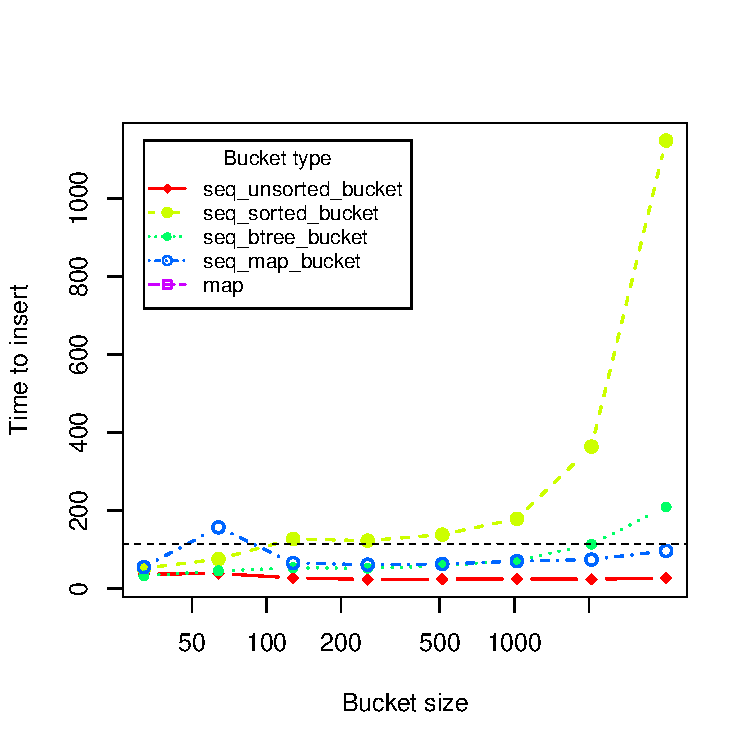
\includegraphics[width=1.0\textwidth]{plots/i7_30m_insert}
        }
        \subfloat[Search]{
            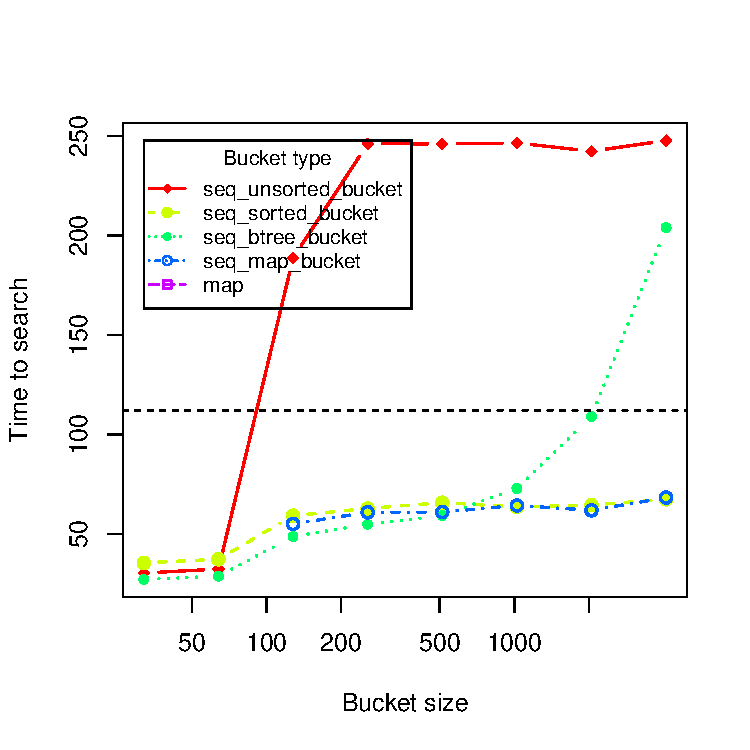
\includegraphics[width=1.0\textwidth]{plots/i7_30m_search}
        }
        \caption{Scaling of insertion and self-search times using the 30M Random
        dataset, with varying bucket sizes from 32 to 4096. The {\keyword map} time
        is shown for reference as a dotted line.}
        \label{fig:seq_30m}
    \end{figure*}
\end{landscape}



\section{Parallel scaling}
In testing the parallel scaling of the different burst trie variants,
a  

Locking improvement: per-node lock.

Amdahls law.


\subsection{Datasets}


These tests show a clear bottleneck already beginning to show at 2 cores for
insertions, while the concurrent locking on insertions allows full parallelism
to the order of the number of cores available. This is caused by the shallow
trie, which is an issue due to node-level parallelism.

Due to sharing of the locks, that needs to be synchronized between caches, on
an expensive interconnect, the scaling is negative. That is, the overhead
created by synchronization of the node locks is greater than the gain in
parallelism.

\begin{table}[h]
    \centering
    \begin{tabular}[here]{ l l l l }
    \hline
        Bucket type            & Size & Insert & Search\\\hline
        %
        STL::Map               & 256  & 1.768  & 5.441\\
        Sorted dynamic array   & 256  & 3.301  & 5.261\\
        Unsorted dynamic array & 64   & 1.030  & 3.644\\
        Unsorted dynamic array & 128+ & ~0.600 & 6.108\\
        Binary tree            & 128  & 1.523  & 4.938\\
        Binary tree            & 32   & 0.979  & 5.680\\
    \hline
    \end{tabular}
    \caption{Speedup factor for each bucket in the 30M dataset for 32 threads on the i7
quad-core machine (virtual octo-core).}
    \label{tab:speedups_30m_i7}
\end{table}

This shows that it is possible to obtain speedup factors of up to 6 with a
fully concurrent locking mechanism. With this as the reference, the gains
of a factor $3.3$ on insertions and a factor $5.2$ on searches, the sorted
dynamic arrays seem to scale the best.

The greatest gains appearing from unsorted array concurrency is evidence that
the locking favors heavy work the leaves. This fits perfectly with the expected
node-level parallelism, which also explains why the greatest gains in insertion
is seen with sorted arrays, being the only bucket structure with linear insertion
times, and thereby up to $O(n^2)$ bursting times.

It is somewhat surprising that the searches take such a big hit from the locking,
evident in the larger unsorted array cases. The empirical concurrency of the
read-locks is hereby reduced. The difference is even greater on the Xeon machine,
where the maximum speedup factor observed for searching was 4.1.


\bibliographystyle{plain}
\bibliography{bibliography}

\end{document}
